We report results over \TotalEvals{} evaluations covering \TotalModels{} models, two GPUs, and \TotalProblems{} problems. Overall, \OverallPassRate\% of runs pass correctness and \OverallBeatRate\% beat the baseline. The average speedup among correct kernels is \AvgSpeedup{}x over \SpeedupCount{} successful runs.

\begin{figure}[t]
\centering
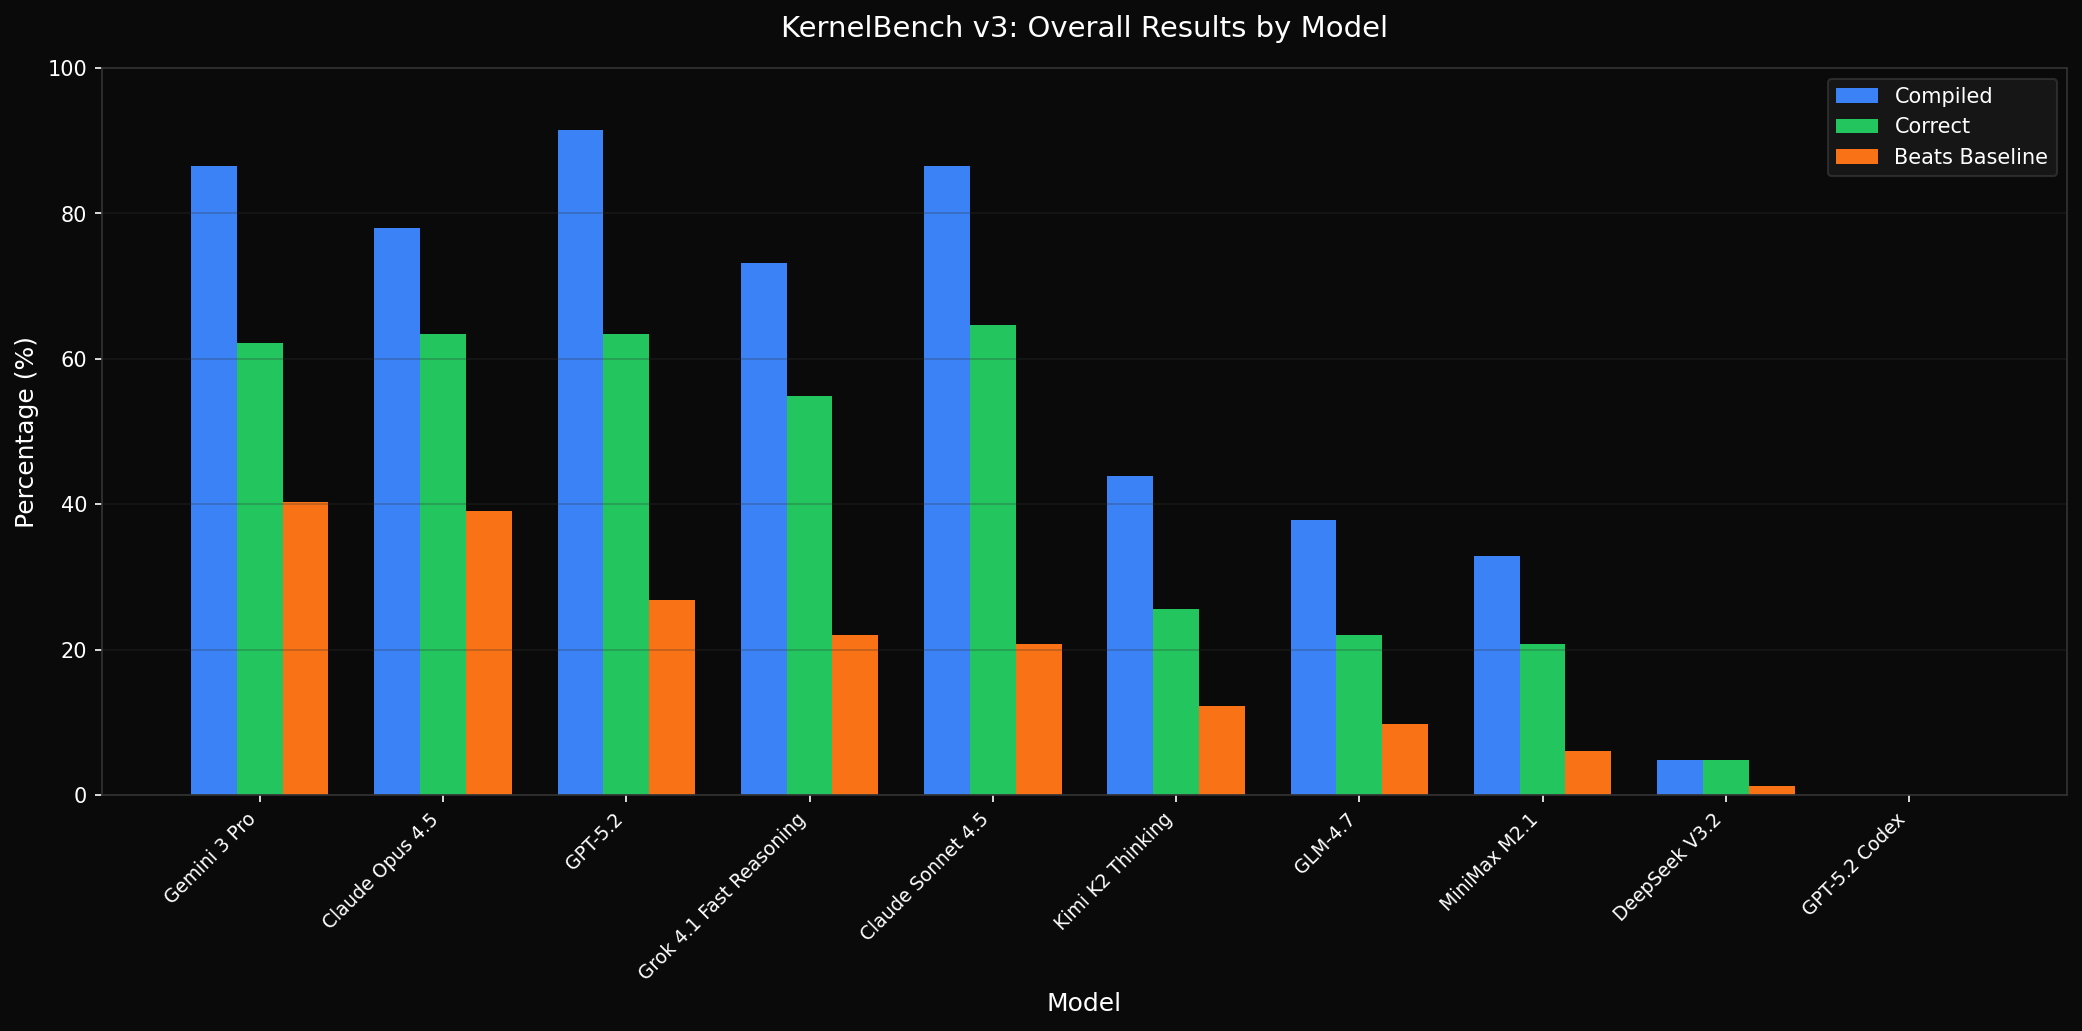
\includegraphics[width=0.95\linewidth]{figures/results_overall.png}
\caption{Overall results by model. Bars show the fraction of runs that compiled, were correct, and beat the baseline.}
\label{fig:overall}
\end{figure}

\noindent Figure~\ref{fig:overall} is sourced from the public dashboard export. GPT-5.2 Codex appears at 0\% there because the evaluation failed due to an API format mismatch in the OpenAI Codex endpoint, not model performance. We exclude GPT-5.2 Codex from the tables and aggregate statistics.

\begin{figure}[t]
\centering
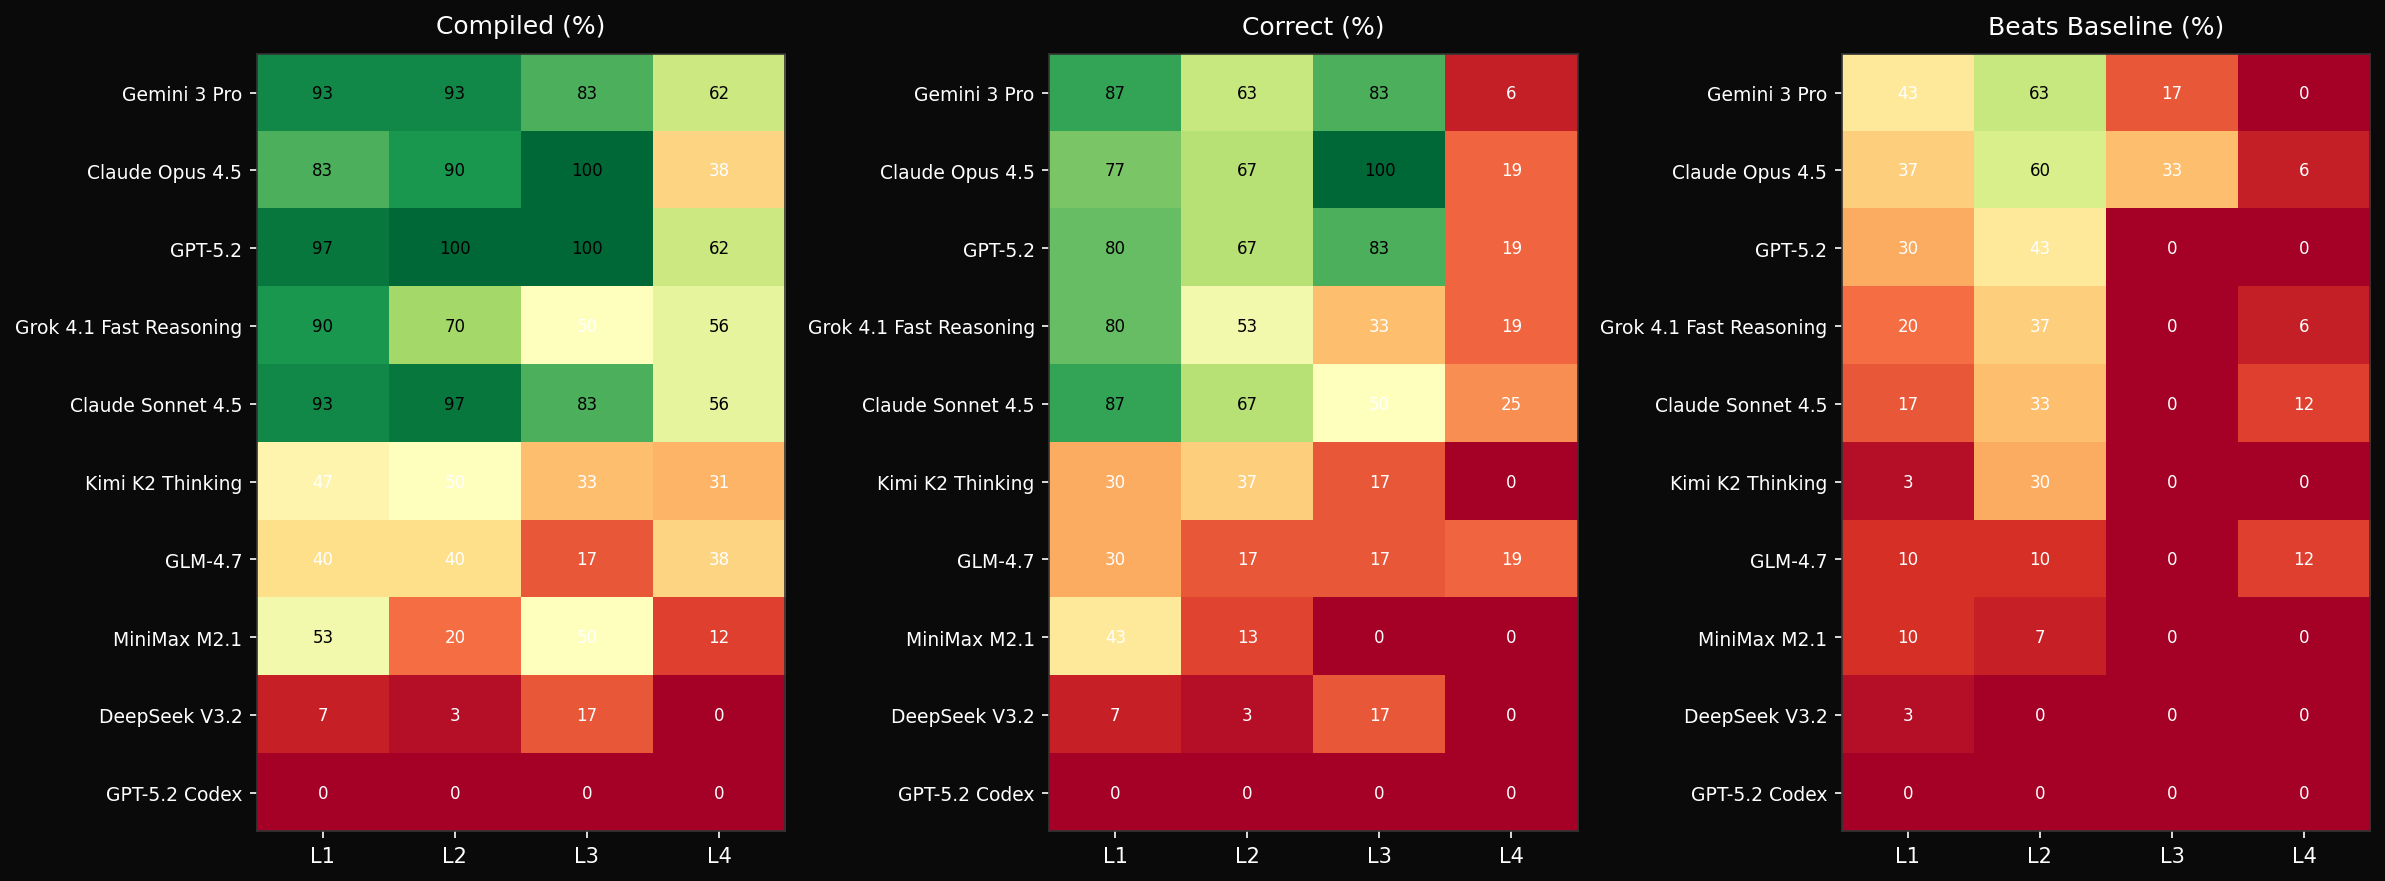
\includegraphics[width=0.98\linewidth]{figures/results_heatmap.png}
\caption{Heatmap of correctness and baseline-beating rates by level.}
\label{fig:heatmap}
\end{figure}

Table~\ref{tab:model-results} summarizes performance by model. Gemini 3 Pro and Claude Opus 4.5 produce the most baseline-beating kernels. GPT-5.2 has strong correctness but fewer baseline wins, indicating that correctness alone does not guarantee competitive performance.

The figures are sourced from the public dashboard export. GPT-5.2 Codex appears at 0\% there because the evaluation failed due to an API format mismatch in the OpenAI Codex endpoint, not model performance. We exclude GPT-5.2 Codex from the tables and aggregate statistics.

\begin{table}[t]
\centering
\caption{Model-level results across all problems and GPUs.}
\label{tab:model-results}
% Auto-generated from results.csv
\begin{tabular}{lrrrr}
\toprule
Model & Correct (\%) & Beat baseline (\%) & Beat baseline (n) & Total \\
\midrule
Gemini 3 Pro & 62.2 & 40.2 & 33 & 82 \\
Claude Opus 4.5 & 63.4 & 39.0 & 32 & 82 \\
GPT-5.2 & 63.4 & 26.8 & 22 & 82 \\
Grok 4.1 Fast Reasoning & 54.9 & 22.0 & 18 & 82 \\
Claude Sonnet 4.5 & 64.6 & 20.7 & 17 & 82 \\
Kimi K2 Thinking & 25.6 & 12.2 & 10 & 82 \\
GLM-4.7 & 22.0 & 9.8 & 8 & 82 \\
MiniMax M2.1 & 20.7 & 6.1 & 5 & 82 \\
DeepSeek V3.2 & 4.9 & 1.2 & 1 & 82 \\
\bottomrule
\end{tabular}

\end{table}

Table~\ref{tab:level-results} breaks down performance by difficulty level. Pass rates decline sharply at Level 4: only \PassRateLFour\% of runs pass correctness and \BeatRateLFour\% beat the baseline. These tasks include modern attention variants and quantized matmuls, and some use already-optimized Triton baselines.

\begin{table}[t]
\centering
\caption{Results by difficulty level.}
\label{tab:level-results}
% Auto-generated from results.csv
\begin{tabular}{crrrr}
\toprule
Level & Pass rate (\%) & Beat baseline (\%) & Beat baseline (n) & Total \\
\midrule
L1 & 57.8 & 19.3 & 52 & 270 \\
L2 & 43.0 & 31.5 & 85 & 270 \\
L3 & 44.4 & 5.6 & 3 & 54 \\
L4 & 11.8 & 4.2 & 6 & 144 \\
\bottomrule
\end{tabular}

\end{table}
